\documentclass[14pt]{extarticle}
\usepackage[english, russian]{babel}
\usepackage[utf8]{inputenc}
\usepackage[T2A]{fontenc}
\usepackage{changepage}
\usepackage{graphicx}
\usepackage{hyperref}
\usepackage{titlesec}
\usepackage{setspace}
\usepackage{hyperref}
\usepackage{amsmath}
\usepackage{tocloft}
\usepackage{caption}
\usepackage{amssymb}
\usepackage{minted}

\usepackage[a4paper, left=2.5cm, right=1.5cm, top=2cm, bottom=3cm]{geometry}

\graphicspath{
    {assets}
}

\onehalfspacing

\titlespacing{\section}{0pt}{3.5pt}{1pt}

\titlespacing{\subsection}{0pt}{3.5pt}{1pt}

\setcounter{tocdepth}{2}

\renewcommand{\cftsecleader}{\cftdotfill{\cftdotsep}}

\begin{document}

\setcounter{secnumdepth}{0}

\thispagestyle{empty}
\begin{titlepage}
    \begin{center}
        МИНОБРНАУКИ РОССИИ\\
        федеральное государственное автономное образовательное\\
        учреждение высшего образования\\
        <<Омский государственный университет им. Ф.М. Достоевского>>\\
        Кафедра компьютерной математики и программного обеспечения\\
        
        \bigskip
        \bigskip
        \bigskip
        
        \begin{adjustwidth}{10cm}{}
            УТВЕРЖДАЮ\\
            И. о. заведующего кафедрой\\
            \rule{3cm}{0.4pt} Симанчёв Р.Ю.\\
            \bigskip
            <<\rule{1cm}{0.4pt}>> \rule{3cm}{0.4pt} 2025 г.\\
        \end{adjustwidth}
        
        \bigskip
        \bigskip
        \bigskip
        
        \textbf{РАЗРАБОТКА КЛИЕНТ-СЕРВЕРНОГО ПРИЛОЖЕНИЯ}\\
        \textbf{ДЛЯ АРЕНДЫ ВЕЩЕЙ}\\
        
        \bigskip
        \bigskip
        
        Выпускная квалификационная работа\\
        по направлению подготовки бакалавров\\
        01.03.02 Прикладная математика и информатика\\
        
        \bigskip
        \bigskip
        \bigskip
        \bigskip
        \bigskip
        \bigskip

        \begin{adjustwidth}{10cm}{}
            Научный руководитель:\\
            к.ф.-м.н., доцент\\
            \rule{3cm}{0.4pt} Ашаева Ю. М.\\
            \bigskip
            <<\rule{1cm}{0.4pt}>> \rule{3cm}{0.4pt} 2025 г.\\
            \bigskip
            \bigskip
            Выполнил:\\
            студент группы ММБ-104-О-02\\
            \rule{3cm}{0.4pt} Карабалин Р. Т.\\
            \bigskip
            <<\rule{1cm}{0.4pt}>> \rule{3cm}{0.4pt} 2025 г.\\
        \end{adjustwidth}

        \bigskip
        \bigskip
        \bigskip
        \bigskip
        \bigskip
        \bigskip

        Омск, 2025
    \end{center}
\end{titlepage}

\newpage

\setcounter{page}{2}
\tableofcontents
\newpage


\section{Введение}

\bigskip

В современном мире, где концепция устойчивого потребления и экономики
совместного использования набирает всё большую популярность,
веб-платформы для аренды вещей становятся неотъемлемой частью
цифровой трансформации.
Данная работа посвящена разработке веб-сайта,
который позволяет пользователям арендовать различные товары,
от бытовой техники до спортивного инвентаря,
минимизируя при этом негативное воздействие на окружающую среду.\\

В условиях растущего спроса на аренду вещей,
традиционные модели бизнеса сталкиваются с рядом вызовов,
таких как необходимость в удобных сервисах,
предоставляющих возможность размещать объявления о товарах доступных для аренды.\\

Целью работы является создание веб-сайта, который не только
удовлетворяет потребности пользователей в аренде вещей,
но и способствует развитию экономики совместного использования,
предоставляя владельцам возможность монетизировать свои активы.
В рамках диплома будут рассмотрены ключевые аспекты проектирования,
разработки веб-приложения.\\

\newpage


\section{Глава 1. Постановка задачи}

\subsection{1.1 Постановка задачи}

\bigskip

Цель работы - разработать клиент-серверное приложение для аренды вещей.\\

Основной функционал приложения состоит в возможности создания объявления
с товаром, доступным для аренды и арендовать товары, которые разместили другие пользователи.
Сервис будет предоставлять пользователям возможность найти нужные им вещи
и уже отдельно самостоятельно связываться друг с другом.\\

Задачи работы:
\begin{enumerate}

    \item Проектирование веб-сайта:
    \begin{enumerate}
        \item Разработать структуру и функциональность веб-сайта.
        \item Определить ключевые пользовательские сценарии и потоки взаимодействия.
        \item Создать прототипы пользовательского интерфейса.
    \end{enumerate}
    
    \item Техническая реализация:
    \begin{enumerate}
        \item Выбрать технологии и инструменты для разработки.
        \item Реализовать основные функции веб-сайта, включая:
        \begin{enumerate}
            \item Регистрацию и аутентификацию пользователей.
            \item Размещение и поиск объявлений о вещах.
            \item Систему бронирования.
        \end{enumerate}
    \end{enumerate}

\end{enumerate}

\newpage


\subsection{1.2 Требования к системе}

\bigskip

Общие требования:
\begin{enumerate}

    \item Регистрация и аутентификация пользователей:
    \begin{enumerate}
        \item Регистрация новых пользователей с помощью email.
        \item Вход в систему с использованием email и пароля.
    \end{enumerate}

    \item Управление профилем:
    \begin{enumerate}
        \item Редактирование личной информации (имя, контактные данные).
        \item Управление фотографией профиля.
        \item Просмотр истории аренд и размещённых объявлений.
    \end{enumerate}

    \item Размещение и управление объявлениями:
    \begin{enumerate}
        \item Загрузка фотографий и описание вещи.
        \item Указание цены аренды за разные временные промежутки.
    \end{enumerate}

    \item Поиск и бронирование:
    \begin{enumerate}
        \item Поиск вещей по ключевым словам.
        \item Возможность бронирования вещи с указанием даты и времени
            начала и конца аренды.
    \end{enumerate}
    
\end{enumerate}

\bigskip

Требования к серверной части приложения:
\begin{enumerate}
    \item Монолитная архитектура.
    \item Использование реляционной базы данных для хранения
        структурированных данных.
    \item Использование отдельного специализированного хранилища объектов
        для хранения изображений.
    \item Обработка ошибок и оповещение о них пользователя.
\end{enumerate}

\newpage

Требования к клиентской части приложения:
\begin{enumerate}
    \item Наличие всех необходимых для работы страниц.
    \item Осуществление простой навигации между доступными страницами.
    \item Наличие понятных форм ввода данных.
    \item Обработка ошибок и оповещение о них пользователя.
\end{enumerate}

\bigskip

Эти требования помогут обеспечить разработку надёжной,
безопасной и удобной веб-платформы для аренды вещей,
которая будет отвечать потребностям пользователей и
способствовать развитию экономики совместного использования.

\newpage

\subsection{1.3 Анализ требований}

\bigskip

Перед началом разработки был проведён анализ требований и
описан функционал, который нужно будет реализовать.

Описание функционала выполнено в формате пользовательских историй
``как \textit{<роль>}, я хочу \textit{<что-то>}, чтобы \textit{<делать что-то>}''.\\

Например:
\begin{enumerate}
    \item Как анонимный пользователь, я хочу зарегистрироваться, чтобы пользоваться веб-сайтом.
    \item Как зарегистрированный пользователь, я хочу создавать объявления, чтобы сдавать свои вещи в аренду.
    \item Как владелец объявления, я хочу редактировать его, чтобы обновлять информацию.
    \item Как зарегистрированный пользователь, я хочу иметь возможность оформить бронь на чужое объявление, чтобы взять вещь в аренду.
\end{enumerate}


Также был разработан основной путь пользователя,
отдельно для владельца вещи и для заказчика
--- того кто хочет арендовать вещь (см. рис. 1).

\begin{center}
    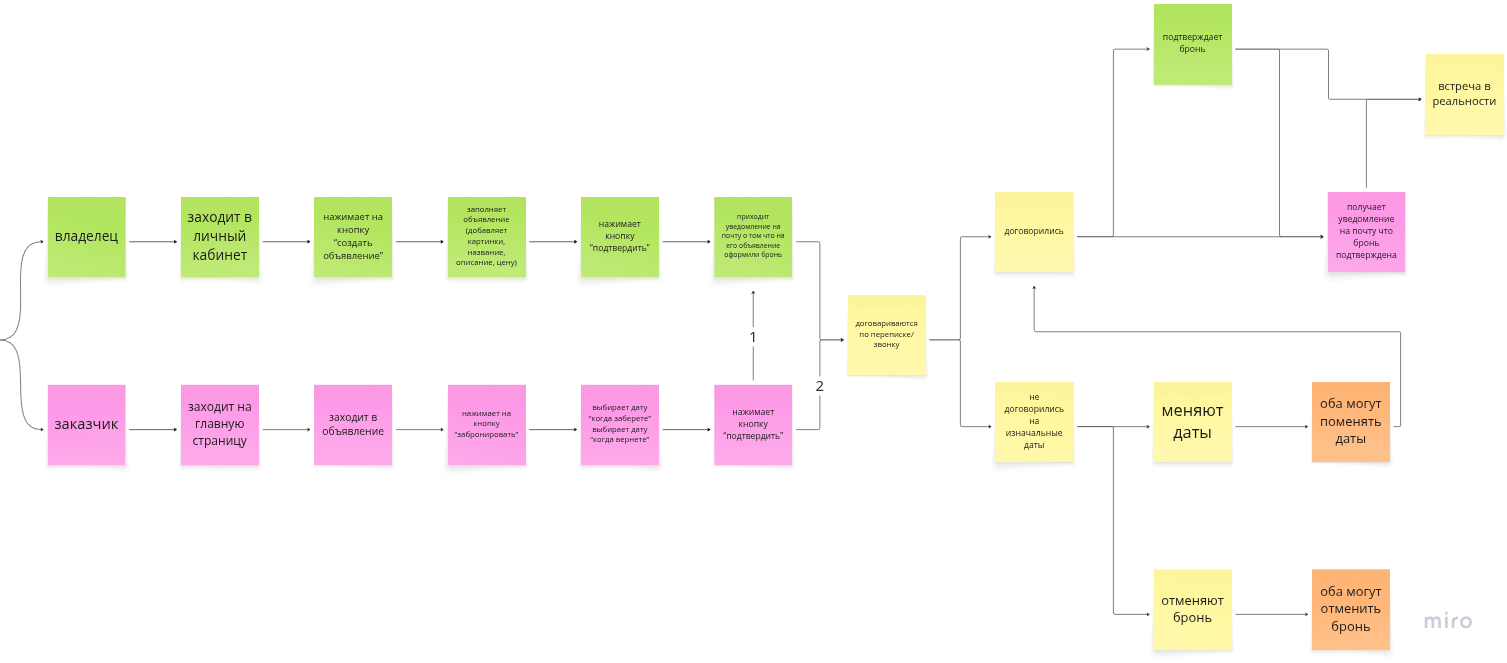
\includegraphics[width=0.7\textwidth]{flow.png}
    \captionof{figure}{}
\end{center}

\newpage

\section{Глава 2. Архитектура приложения}

\subsection{2.1 Серверная часть приложения}

\subsection{2.1.1 Используемые технологии}

\bigskip

Серверная часть приложения разрабатывалась с использованием
следующих технологий:
\begin{enumerate}
    \item Язык программирования Kotlin.
    \item Фреймворк для создания веб-приложений Spring Boot 3.
    \item Контейнеризатор приложений Docker.
    \item Инструмент для управления и автоматизации изменений
        схемы базы данных Liquibase.
    \item Реляционная база данных PostgreSQL.
    \item Облачное хранилище файлов Yandex Object Storage.
\end{enumerate}

\bigskip

Язык Kotlin был выбран для разработки благодаря ряду преимуществ.
Во-первых, он предоставляет удобные средства сборки,
которые упрощают процесс создания и управления проектами.
Во-вторых, Kotlin обеспечивает безопасность типов,
что помогает минимизировать ошибки на этапе компиляции
и повышает надежность кода.
В-третьих, язык обладает растущей популярностью и востребованностью на рынке,
что делает его востребованным среди специалистов и перспективным для бизнеса,
что обеспечивает широкую поддержку сообщества и доступ к современным библиотекам.

\bigskip

Для хранения изображений я использую Yandex Object Storage,
этот подход предпочтительнее, поскольку хранение картинок в PostgreSQL
будет замедлять работу базы данных, в то время как используемое мной решение
специально предназначено для хранения файлов, что позволяет хранить большое количество
изображений не теряя производительность основной базы данных.

\subsection{2.1.2 Архитектура приложения}

\bigskip

Серверная часть приложения представляет API,
реализованое с использованием архитектурного стиля REST.

\bigskip

\textbf{API (application programming interface)} --- описание способов (набор
классов, процедур, функций, структур или констант), которыми одна
программа может взаимодействовать с другой программой.

\bigskip

\textbf{REST (Representational state transfer)} --- это архитектурный стиль
взаимодействия компонентов распределенного приложения в сети, для
которого характерны следующие ограничения:
\begin{itemize}
    \item применимость в клиент-серверной архитектуре
    \item вся информация, необходимая для обработки запроса, должна
        содержаться в самом запросе
    \item доступ должен предоставляться только через URL
\end{itemize}

\bigskip

Клиент общается с сервером с помощью HTTP-запросов (см. рис. 2),
данные, как правило, передаются в виде JSON-строк.
Часть данных может передаваться через параметры URL или через сам URL.

\begin{center}
    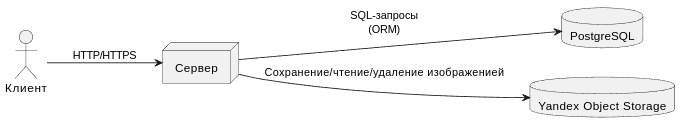
\includegraphics[width=0.8\textwidth]{client-server.png}
    \captionof{figure}{}
\end{center}

\bigskip

Серверная часть приложения имеет привычную архитектуру,
представленную тремя слоями: контроллеров, сервисов и репозиториев.

Контроллер принимает на вход запрос, возможно как-то преобразует его
и передаёт сервису (см. рис. 3). После обработки данных сервисом, контроллер
формирует HTTP-ответ на основе результата работы сервиса.

\begin{center}
    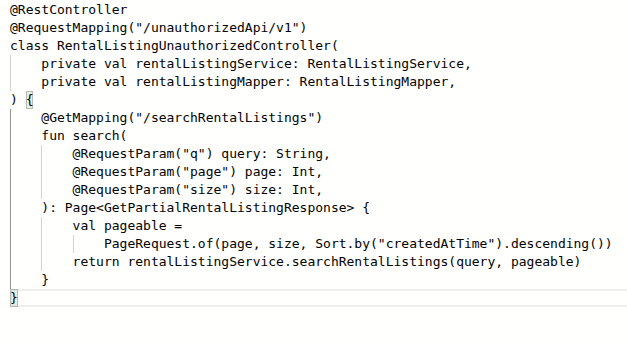
\includegraphics[width=1.0\textwidth]{controller.png}
    \captionof{figure}{Пример контроллера}
\end{center}

Сервис принимает на вход данные, как-то преобразует их, обращается к репозиториям
если нужны какие-то дополнительные данные, агрегирует данные и возвращает
новые данные (см. рис. 4).

\begin{center}
    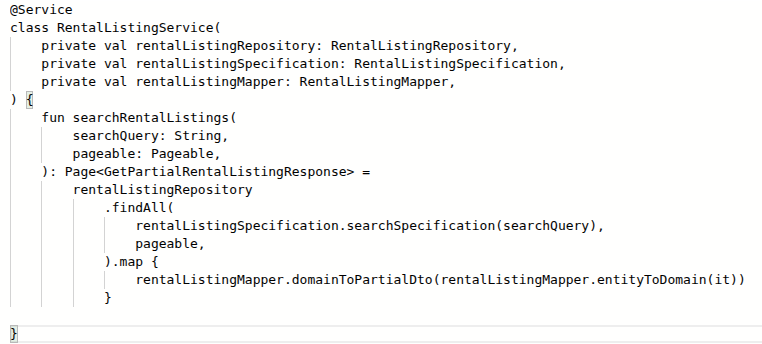
\includegraphics[width=1.0\textwidth]{service.png}
    \captionof{figure}{Пример сервиса}
\end{center}

Из-за использования Spring Data JPA, репозитории представляют из себя
интерфейсы, которые наследуют контракты от интерфейса JpaRepository,
который предоставляет базовые запросы к базе данных, но в некоторых случаях
мне понадобились специфические запросы, которые я реализовал на чистом SQL
(см. рис. 5).

\begin{center}
    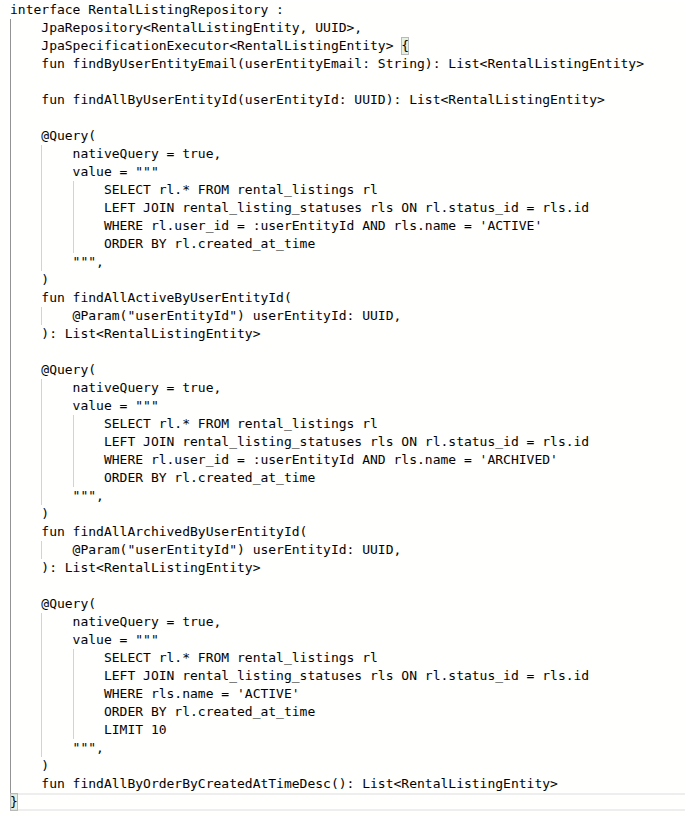
\includegraphics[width=1.0\textwidth]{repository.png}
    \captionof{figure}{Пример репозитория}
\end{center}

\newpage

\subsection{2.1.3 Хранилища данных}

\bigskip

Для обеспечения эффективной работы серверной части приложения используются
два основных типа хранилищ данных: реляционная база данных
PostgreSQL для хранения структурированных данных
и облачное хранилище Yandex Object Storage
для хранения неструктурированных данных, таких как изображения.
Эти хранилища были выбраны с учетом их производительности,
масштабируемости и соответствия требованиям проекта.
Ниже представлено подробное описание каждого из них.

PostgreSQL --- это мощная, открытая реляционная система управления
базами данных (СУБД), которая используется в проекте для хранения
структурированных данных, таких как информация о пользователях,
объявлениях, арендах.

В приложении PostgreSQL используется для хранения всех данных,
необходимых для бизнес-логики, за исключением файлов изображений.
Схема базы данных проектируется с учетом нормализации
для минимизации избыточности данных и обеспечения эффективных запросов.

Для управления схемой базы данных применяется Liquibase,
который автоматизирует миграции базы данных.
Liquibase хранит историю изменений схемы в виде YAML-файлов,
что позволяет синхронизировать структуру
базы данных между различными окружениями
и откатывать изменения при необходимости.

Yandex Object Storage --- это облачное объектное хранилище,
которое используется для хранения изображений, загружаемых пользователями.
Выбор данного хранилища обусловлен его производительностью
и экономичностью по сравнению с хранением файлов непосредственно
в реляционной базе данных.

Изображения загружаются в Yandex Object Storage через REST API.
После успешной загрузки файла уникальный идентификатор сохраняется в базу данных PostgreSQL.
Такой подход позволяет разделить хранение самих файлов и их метаданных,
что повышает производительность базы данных, так как PostgreSQL
не перегружается большими бинарными данными.
Кроме того, использование объектного хранилища упрощает доступ к файлам
через прямые URL-адреса, что удобно для клиентской части приложения.

Для работы с облачным хранилищем используется AWS SDK,
который интегрируется с приложением и позволяет программно
загружать и управлять файлами.

Схема базы данных представлена на рисунке 6.

\begin{center}
    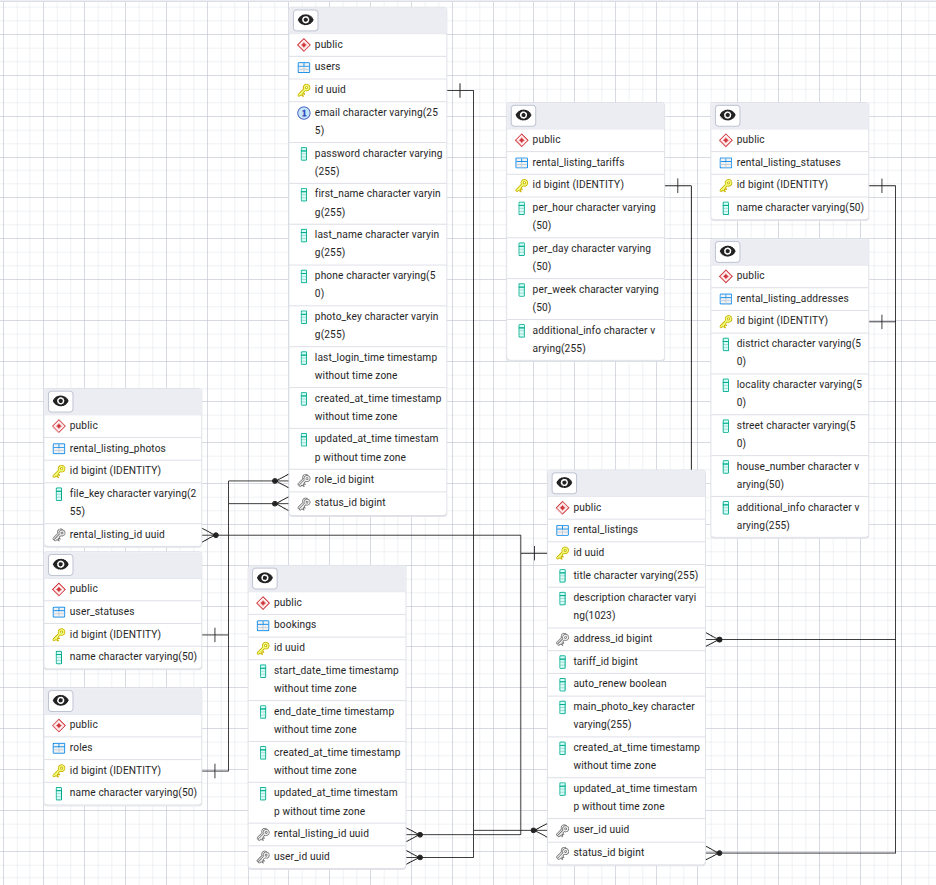
\includegraphics[width=1.0\textwidth]{erd.png}
    \captionof{figure}{}
\end{center}

Поля \textit{users.photo\_key}, \textit{rental\_listings.main\_photo\_key} и
\textit{rental\_listing\_photos.file\_key} содержат ключи, которые являются
идентификаторами картинок в Yandex Object Storage, на рисунке 7 показано как выглядит панель просмотра хранилища.

\begin{center}
    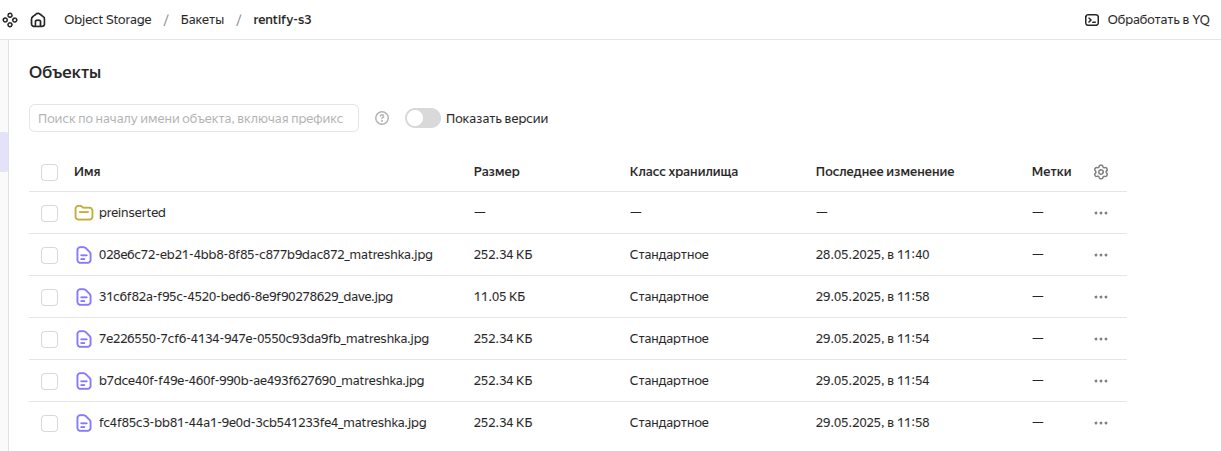
\includegraphics[width=1.0\textwidth]{ys3.png}
    \captionof{figure}{}
\end{center}


\subsection{2.2 Клиентская часть приложения}

\bigskip

Для разработки клиентской части приложения использовались
следующих технологий:
\begin{enumerate}
    \item Язык программирования TypeScript.
    \item Фреймворк для создания веб-приложений React.
    \item Библиотека для работы с состоянием приложения Redux, Redux Toolkit
    \item Коллекция навигационных компонентов React Router
    \item Библиотека компонентов Material UI (MUI)
    \item HTTP-клиент для выполнения запросов на сервер Axios
\end{enumerate}

Основным фреймворком для разработки клиентской части я выбрал react,
так как он позволяет простой и понятный подход создания интерфейсов из компонентов,
которые могут быть переиспользованы в любом другом месте интерфейса.

\bigskip

Для обеспечения удобной навигации использована библиотека react-router.
Она позволяет описывать страницы как отдельные react компоненты,
и легко переключаться между ними, при этом сама страница перезагружаться не будет,
рендеринг будет происходить динамически.

\bigskip

Для работы с данными которые должны храниться независимо от того какая страница сейчас открыта,
использована библиотека redux. Он позволяет объявить единое хранилища,
которое доступно в любом компоненте, что позволяет быстро получить доступ к нужным данным.

\bigskip

Для упрощения сохранения общей стилистики приложения, использована библиотеку компонентов
MUI. Она позволяет не задумываться о том, как будет выглядеть интерфейс, а сосредоточиться
на функциональности.

\bigskip

Для выполнения HTTP-запросов использована библиотека axios,
она позволяет удобно создавать повторно используемые конфигурации,
что упрощает управление HTTP-заголовками и другими параметрами запроса.

\newpage

\section{Глава 3. Описание работы приложения}

Рассмотрим работу с приложением. Когда не аутентифицированный пользователь заходит
на сайт, он видит основную страницу со строкой поиска
и 10 самыми новыми объявлениями (см. рис. 8).

\begin{center}
    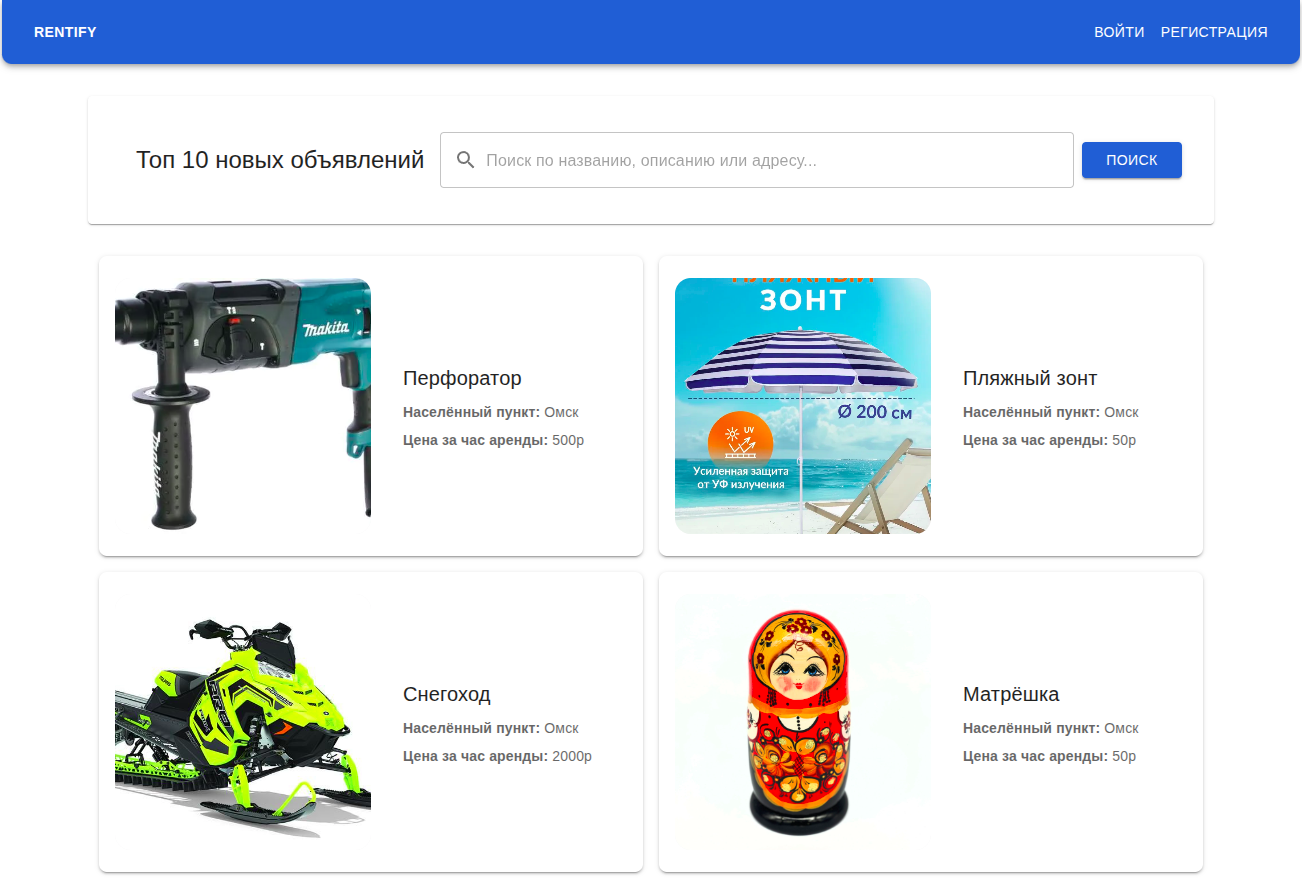
\includegraphics[width=0.7\textwidth]{homePage.png}
    \captionof{figure}{Основная страница}
\end{center}

При нажатии на кнопку ``Регистрация'', открывается страница с формой регистрации
аккаунта (см. рис. 9).

\begin{center}
    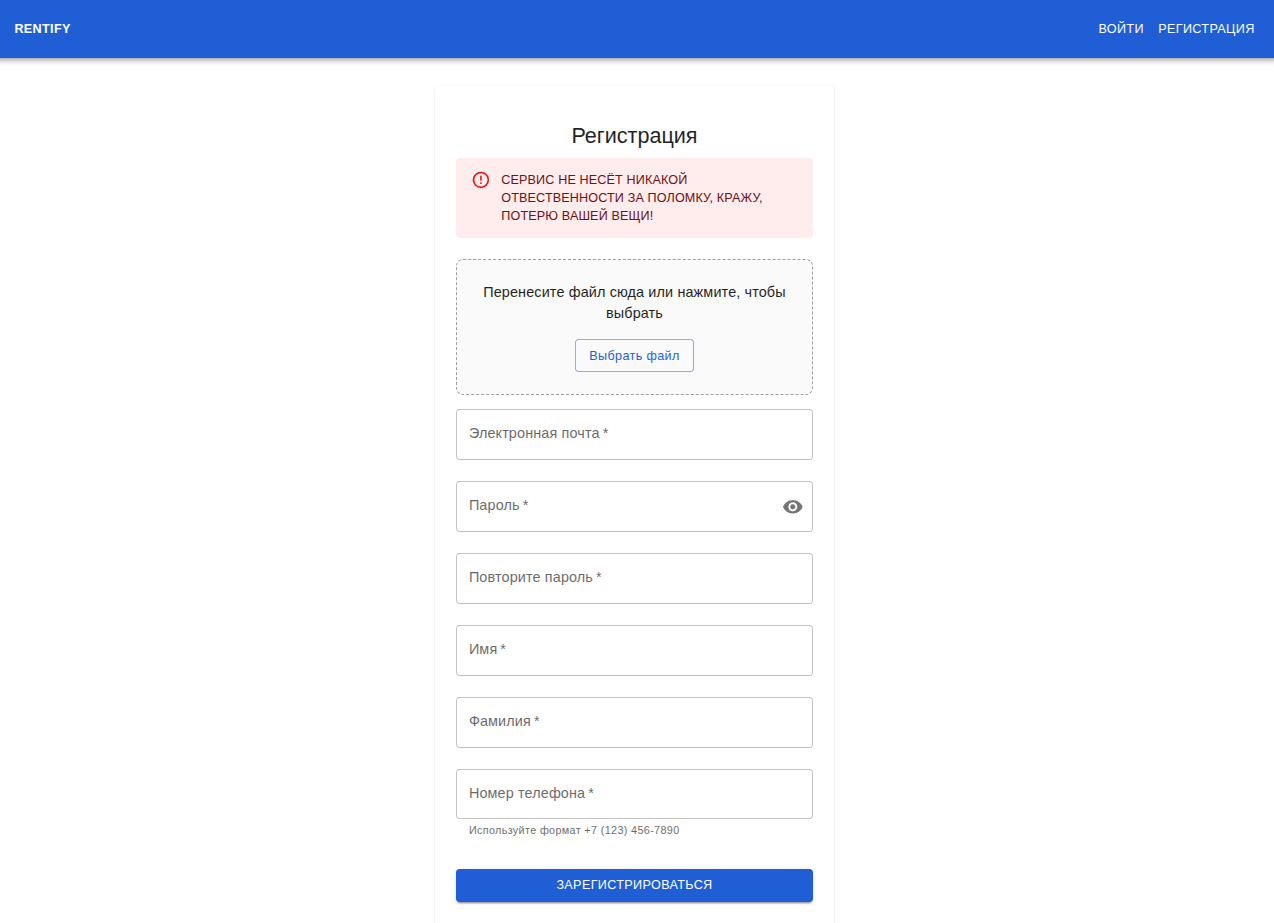
\includegraphics[width=0.7\textwidth]{register.png}
    \captionof{figure}{Страница регистрации}
\end{center}

После регистрации у пользователя появляется доступ в личный кабинет.
Там пользователь может посмотреть основную информацию об аккаунте (см. рис. 10).

\begin{center}
    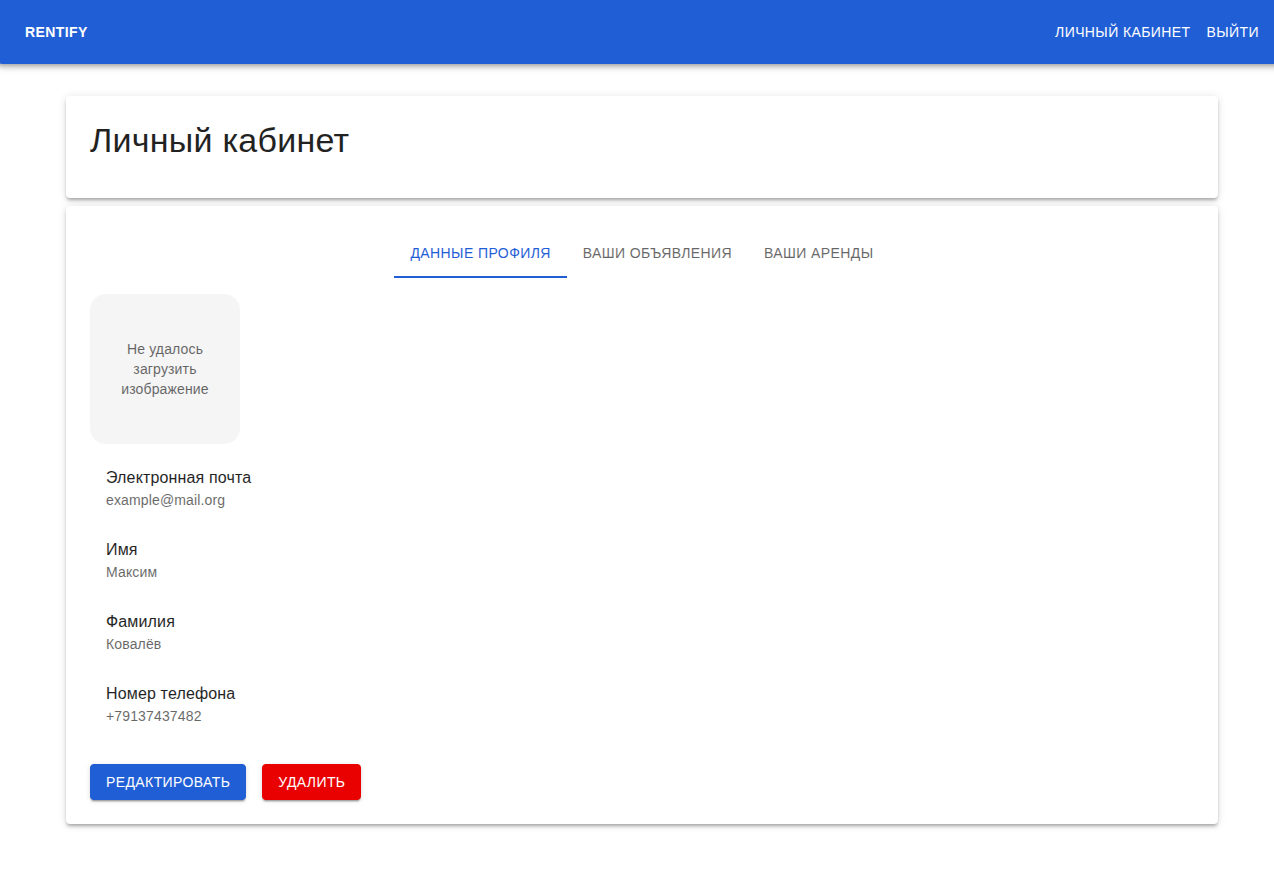
\includegraphics[width=0.7\textwidth]{account.png}
    \captionof{figure}{Личный кабинет}
\end{center}

Рассмотрим функциональность создания объявления.
Во вкладке ``Ваши объявления'' пользователь может создать новое объявление
которое станет доступным для аренды другим пользователям (см. рис. 11).

\begin{center}
    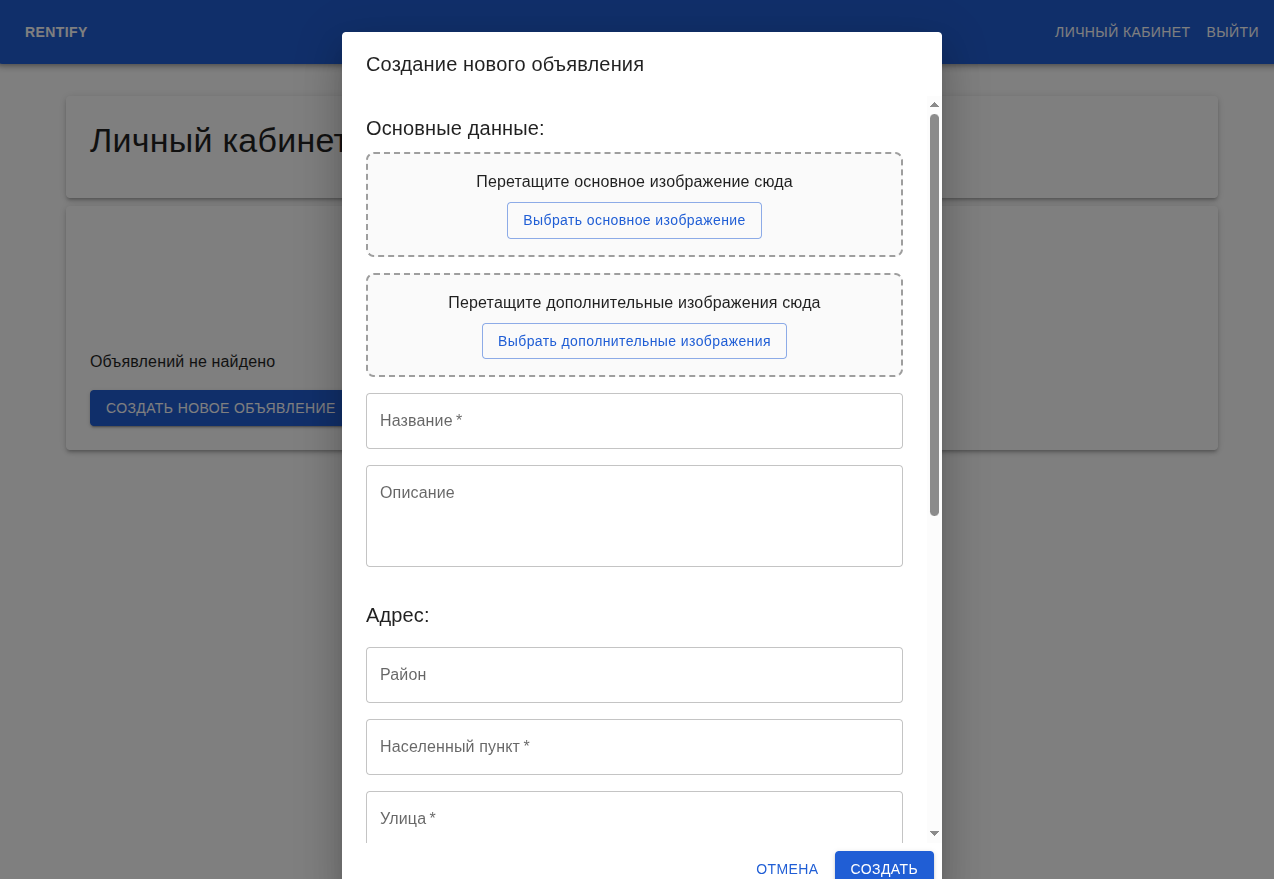
\includegraphics[width=0.7\textwidth]{listings01.png}
    \captionof{figure}{Создание объявления}
\end{center}

После создания, объявление будет отображаться в соотвествующей вкладке.
Также пользователю будет доступно изменения, архивация и удаление объявления
(см. рис. 12). Если кто-либо оформит аренду, соответствующая информация отобразится в объявлении,
вы также можете изменить аренду или отменить её.

\begin{center}
    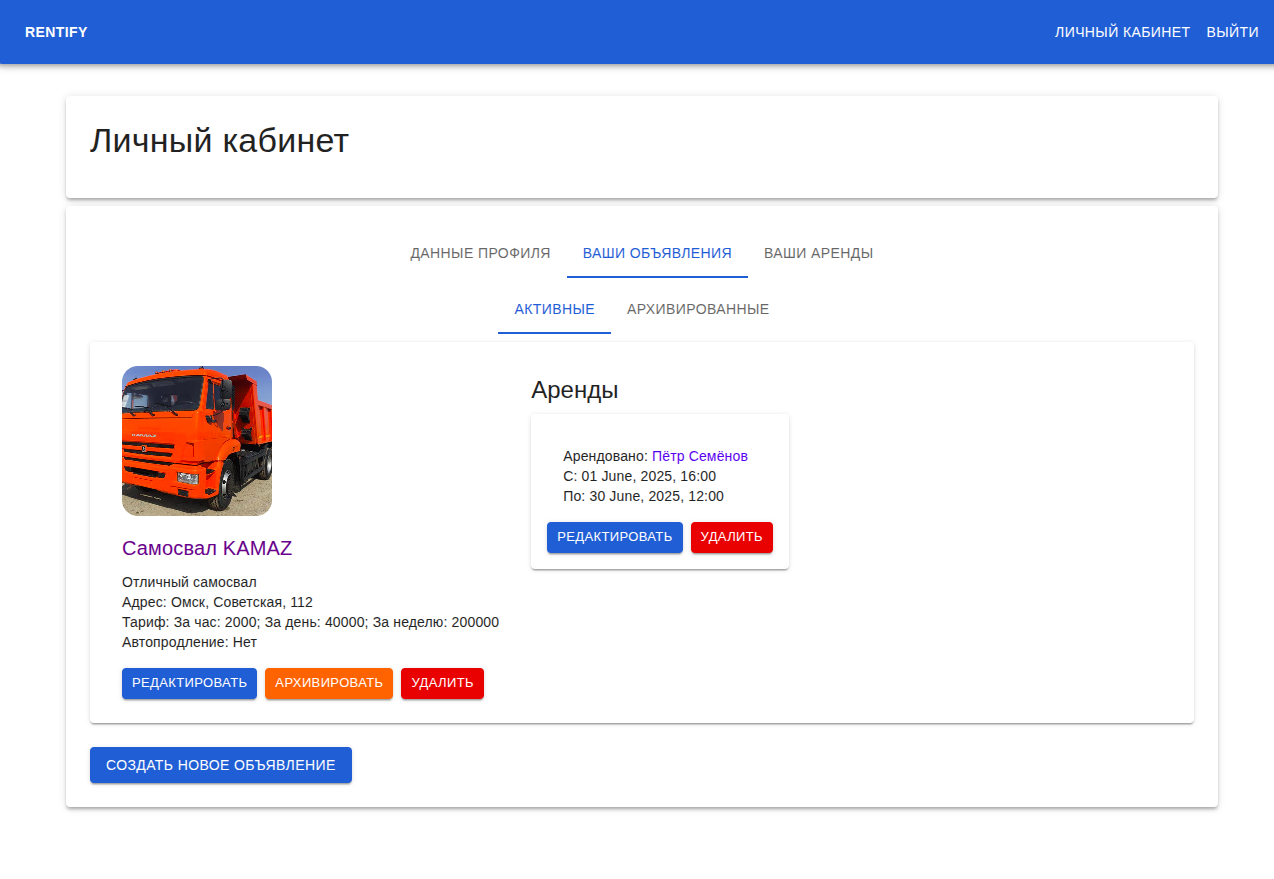
\includegraphics[width=0.6\textwidth]{listings02.png}
    \captionof{figure}{}
\end{center}

Теперь рассмотрим как мы можем оформлять аренду.
Предположим пользователю нужен перфоратор, он ввёл в строку поиска ``Перфоратор''
и нажал кнопку ``Поиск''. Перед ним открылась страница изображенная на рисунке 13.

\begin{center}
    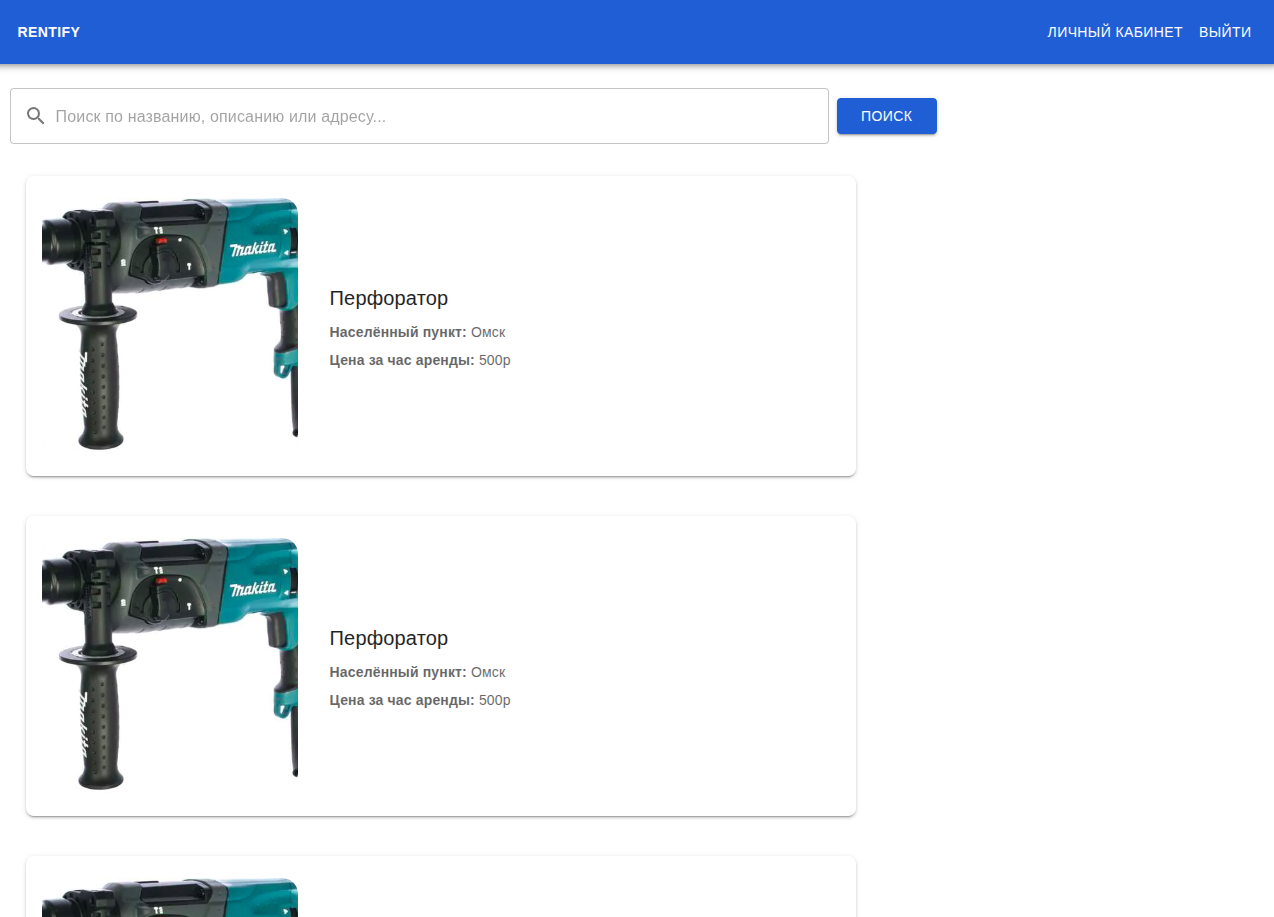
\includegraphics[width=0.6\textwidth]{search.png}
    \captionof{figure}{}
\end{center}

Пользователь открыл интересующее его объявление. Перед ним открывается
страница объявления, изображены картинки объявления, название,
описание, адрес, тариф, а также кто является владельцем вещи (см. рис. 14).

\begin{center}
    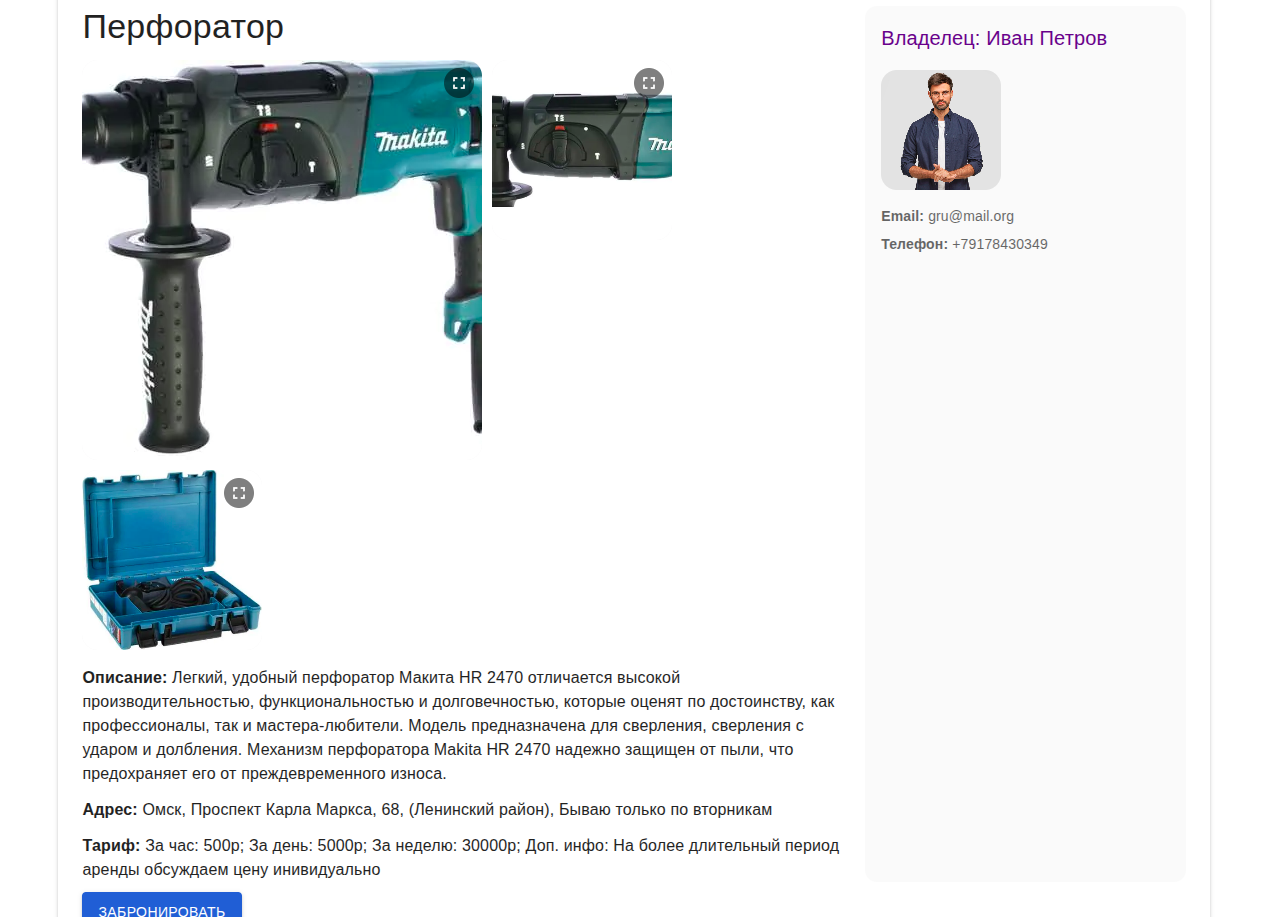
\includegraphics[width=0.6\textwidth]{perforator.png}
    \captionof{figure}{}
\end{center}

При нажатии на кнопку ``Забронировать''. Перед пользователем открывается форма
в которой ему нужно выбрать даты и время начала и конца брони (см. рис. 15).
После этого у владельца будет отображена ваша аренда.
Когда вы оформите аренду, вам нужно будет связаться с владельцем вещи
--- позвонить по номеру телефона или написать на электронную почту.
Также вы и владелец объявления могут редатировать аренду --- менять
даты и время и отменять аренду.

\begin{center}
    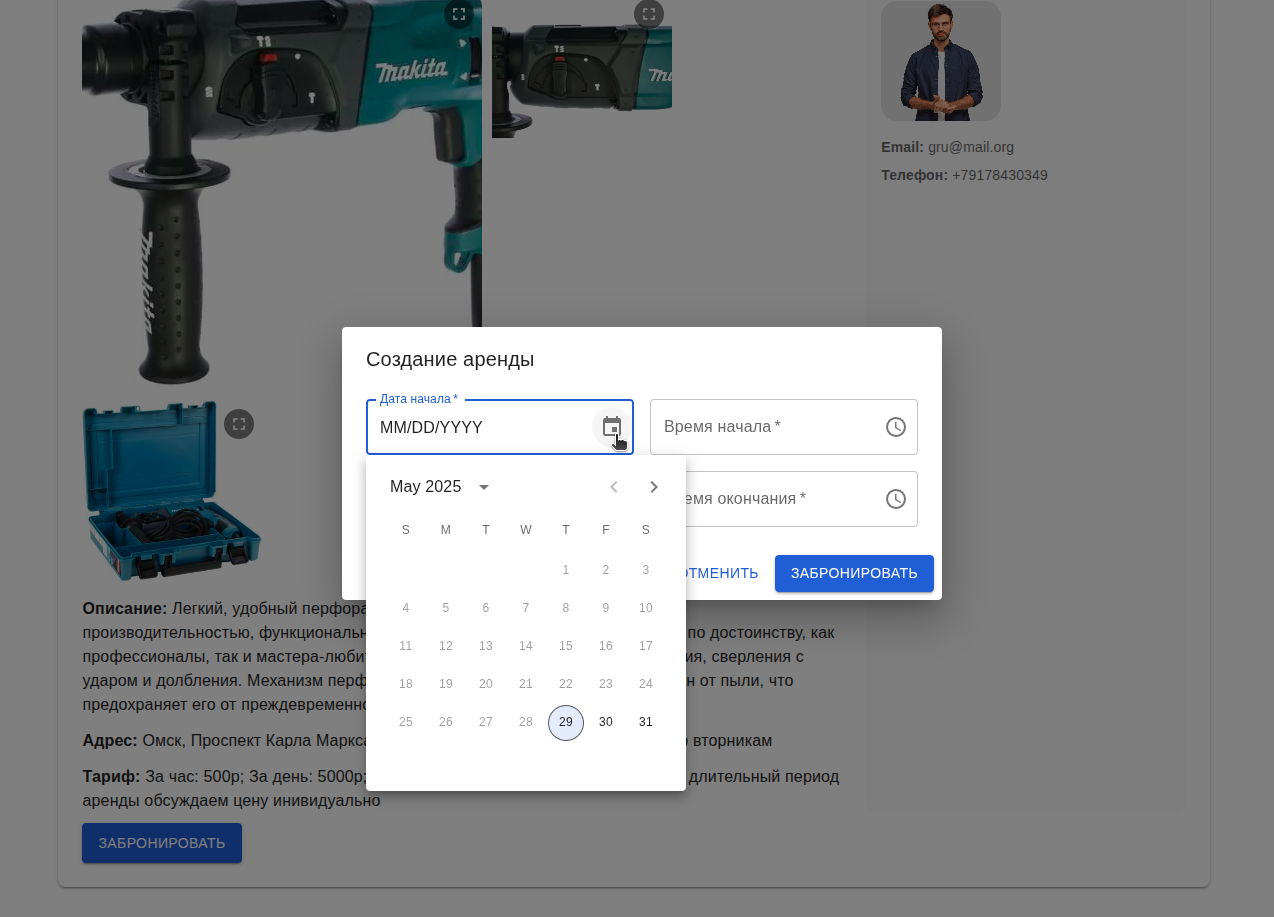
\includegraphics[width=0.5\textwidth]{booking.png}
    \captionof{figure}{}
\end{center}



\newpage


\section{Заключение}

В ходе выполнения работы была достигнута поставленная цель ---
разработано клиент-серверное приложение для аренды вещей,
реализован основной функционал: возможности создания объявления с товаром
доступным для аренды и арендовать товары, которые разместили другие пользователи.

Для достижения этой цели были успешно выполнены все поставленные задачи.
Был проведён анализ требований и составлены базовые сценарии использования сайта.
Была спроектирована схема базы данных, разработаны серверная и клиентская часть приложения
с использование современных технологий, также обеспечена интеграция с облачным хранилищем
Yandex Object Storage для эффективного управления изображениями.

В перспективе платформа может быть расширена за счёт внедрения следующих функций:
добавление внутренних чатов между пользователями, интеграция с платёжными системами,
улучшение поисковых алгоритмов, добавление модерации и администрации,
возможность оставлять отзывы и формировать рейтинг пользователей,
что сделает её ещё более удобной и востребованной.

Разработанное приложение демонстрирует успешное сочетание технических решений
и современных подходов к созданию цифровых продуктов,
способных отвечать актуальным вызовам экономики совместного использования.

\newpage


\section{Список литературы}

\bigskip

\begin{enumerate}
    \item Документация Kotlin. [Электронный ресурс]\\
    Режим доступа: https://kotlinlang.org/docs/home.html\\
    (дата обращения: 08.06.2025)
    
    \item Документация Spring Boot 3. [Электронный ресурс]\\
    Режим доступа: https://docs.spring.io/spring-boot/index.html\\
    (дата обращения: 08.06.2025)
    
    \item Документация PostgreSQL. [Электронный ресурс]\\
    Режим доступа: https://www.postgresql.org/docs\\
    (дата обращения: 08.06.2025)
    
    \item Документация TypeScript. [Электронный ресурс]\\
    Режим доступа: https://www.typescriptlang.org/docs\\
    (дата обращения: 08.06.2025)

    \item Документация React. [Электронный ресурс]\\
    Режим доступа: https://react.dev\\
    (дата обращения: 08.06.2025)

    \item Документация React Router. [Электронный ресурс]\\
    Режим доступа: https://reactrouter.com\\
    (дата обращения: 08.06.2025)

    \item Документация Redux. [Электронный ресурс]\\
    Режим доступа: https://redux.js.org\\
    (дата обращения: 08.06.2025)

    \item Документация MUI. [Электронный ресурс]\\
    Режим доступа: https://mui.com\\
    (дата обращения: 08.06.2025)

    \item Документация axios. [Электронный ресурс]\\
    Режим доступа: https://axios-http.com\\
    (дата обращения: 08.06.2025)

    \item Документация Docker. [Электронный ресурс]\\
    Режим доступа: https://docs.docker.com\\
    (дата обращения: 08.06.2025)

    \item Документация Liquibase. [Электронный ресурс]\\
    Режим доступа: https://docs.liquibase.com/home.html\\
    (дата обращения: 08.06.2025)

    \item Документация AWS SDK. [Электронный ресурс]\\
    Режим доступа: https://docs.aws.amazon.com/sdk-for-java\\
    (дата обращения: 08.06.2025)
\end{enumerate}

\end{document}
